\documentclass[a4paper,oneside,14pt]{extarticle}

\usepackage{cmap} % Улучшенный поиск русских слов в полученном pdf-файле
\usepackage[T2A]{fontenc} % Поддержка русских букв
\usepackage[utf8]{inputenc} % Кодировка utf8
\usepackage[english,russian]{babel} % Языки: русский, английский

\usepackage[14pt]{extsizes}

\usepackage{graphicx}
\usepackage{multirow}

\usepackage{tikz}
\usetikzlibrary{shapes, shapes.geometric, arrows, arrows.meta, positioning}

\usepackage{caption}
\captionsetup{labelsep=endash}
\captionsetup[figure]{name={Рисунок}}

\usepackage{amsmath}
\usepackage{amsfonts}

\usepackage{geometry}
\geometry{left=30mm}
\geometry{right=10mm}
\geometry{top=20mm}
\geometry{bottom=20mm}

\usepackage{enumitem}

\usepackage{tabularx}
\usepackage{longtable}
\usepackage{adjustbox}
\usepackage{threeparttable}

% Переопределение стандартных \section, \subsection, \subsubsection по ГОСТу;
\usepackage{titlesec}[explicit]
\titleformat{name=\section,numberless}[block]{\normalfont\large\bfseries\centering}{}{0pt}{}
\titleformat{\section}[block]{\normalfont\large\bfseries}{\thesection}{1em}{}
\titlespacing\section{\parindent}{*4}{*4}

\titleformat{\subsection}[hang]
{\bfseries\large}{\thesubsection}{1em}{}
\titlespacing\subsection{\parindent}{*2}{*2}

\titleformat{\subsubsection}[hang]
{\bfseries\large}{\thesubsubsection}{1em}{}
\titlespacing\subsubsection{\parindent}{*2}{*2}

\usepackage{url}

% Переопределение их отступов до и после для 1.5 интервала во всем документе
\usepackage{setspace}
\onehalfspacing % Полуторный интервал
\frenchspacing
\setlength\parindent{1.25cm}

\usepackage{indentfirst} % Красная строка

% Настройки оглавления
\usepackage{xcolor}
\usepackage{multirow}

% Гиперссылки
\usepackage[pdftex]{hyperref}
\hypersetup{hidelinks}

% Дополнительное окружения для подписей
\usepackage{array}
\newenvironment{signstabular}[1][1]{
	\renewcommand*{\arraystretch}{#1}
	\tabular
}{
	\endtabular
}

\usepackage{enumitem} 
\setenumerate[0]{label=\arabic*)} % Изменение вида нумерации списков
\renewcommand{\labelitemi}{---}

% Листинги 
\usepackage{courier}
\usepackage{listings}
\usepackage{chngcntr} % Listings counter within section set main.tex after begin document
\usepackage{float} % Place figures anywhere you want; ignore floating
\floatstyle{plaintop}
\newfloat{code}{H}{myc}

% Для листинга кода:
\lstset{
	basicstyle=\small\ttfamily,			% размер и начертание шрифта для подсветки кода
	language=C++,   					% выбор языка для подсветки	
	numbers=left,						% где поставить нумерацию строк (слева\справа)
	numbersep=5pt,
	% stepnumber=1,						% размер шага между двумя номерами строк
	xleftmargin=17pt,
	% showstringspaces=false,
	numbersep=5pt,						% как далеко отстоят номера строк от подсвечиваемого кода
	frame=single,						% рисовать рамку вокруг кода
	tabsize=4,							% размер табуляции по умолчанию равен 4 пробелам
	captionpos=b,						% позиция заголовка вверху [t] или внизу [b]
	breaklines=true,					
	breakatwhitespace=true,				% переносить строки только если есть пробел
	escapeinside={\#*}{*)},				% если нужно добавить комментарии в коде
	inputencoding=utf8x,
	backgroundcolor=\color{white},
	numberstyle=,%\tiny,					    % размер шрифта для номеров строк
	keywordstyle=\color{blue},
	stringstyle=\color{red!90!black}, % color of text in ""
	commentstyle=\color{green!50!black}
}
\lstdefinelanguage[RISC-V]{Assembler}
{
  alsoletter={.}, % allow dots in keywords
  alsodigit={0x}, % hex numbers are numbers too!
  morekeywords=[1]{ % instructions
    lb, lh, lw, lbu, lhu,
    sb, sh, sw,
    sll, slli, srl, srli, sra, srai,
    add, addi, sub, lui, auipc,
    xor, xori, or, ori, and, andi,
    slt, slti, sltu, sltiu,
    beq, bne, blt, bge, bltu, bgeu,
    j, jr, jal, jalr, ret,
    scall, break, nop
  },
  morekeywords=[2]{ % sections of our code and other directives
    .align, .ascii, .asciiz, .byte, .data, .double, .extern,
    .float, .globl, .half, .kdata, .ktext, .set, .space, .text, .word
  },
  morekeywords=[3]{ % registers
    zero, ra, sp, gp, tp, s0, fp,
    t0, t1, t2, t3, t4, t5, t6,
    s1, s2, s3, s4, s5, s6, s7, s8, s9, s10, s11,
    a0, a1, a2, a3, a4, a5, a6, a7,
    ft0, ft1, ft2, ft3, ft4, ft5, ft6, ft7,
    fs0, fs1, fs2, fs3, fs4, fs5, fs6, fs7, fs8, fs9, fs10, fs11,
    fa0, fa1, fa2, fa3, fa4, fa5, fa6, fa7
  },
  morecomment=[l]{;},   % mark ; as line comment start
  morecomment=[l]{\#},  % as well as # (even though it is unconventional)
  morestring=[b]",      % mark " as string start/end
  morestring=[b]'       % also mark ' as string start/end
}
\lstset{
	basicstyle=\small\ttfamily,			% размер и начертание шрифта для подсветки кода
    language=[RISC-V]Assembler,   					% выбор языка для подсветки	
	numbers=left,						% где поставить нумерацию строк (слева\справа)
	numbersep=5pt,
	% stepnumber=1,						% размер шага между двумя номерами строк
	xleftmargin=17pt,
	% showstringspaces=false,
	numbersep=5pt,						% как далеко отстоят номера строк от подсвечиваемого кода
	frame=single,						% рисовать рамку вокруг кода
	tabsize=4,							% размер табуляции по умолчанию равен 4 пробелам
	captionpos=b,						% позиция заголовка вверху [t] или внизу [b]
	breaklines=true,					
	breakatwhitespace=true,				% переносить строки только если есть пробел
	escapeinside={\#*}{*)},				% если нужно добавить комментарии в коде
	inputencoding=utf8x,
	backgroundcolor=\color{white},
	numberstyle=,%\tiny,					    % размер шрифта для номеров строк
	keywordstyle=\color{blue},
	stringstyle=\color{red!90!black}, % color of text in ""
	commentstyle=\color{green!50!black}
}
\lstset{
 morekeywords={size_t, likely}
}

\lstset{
	literate=
	{а}{{\selectfont\char224}}1
	{б}{{\selectfont\char225}}1
	{в}{{\selectfont\char226}}1
	{г}{{\selectfont\char227}}1
	{д}{{\selectfont\char228}}1
	{е}{{\selectfont\char229}}1
	{ё}{{\"e}}1
	{ж}{{\selectfont\char230}}1
	{з}{{\selectfont\char231}}1
	{и}{{\selectfont\char232}}1
	{й}{{\selectfont\char233}}1
	{к}{{\selectfont\char234}}1
	{л}{{\selectfont\char235}}1
	{м}{{\selectfont\char236}}1
	{н}{{\selectfont\char237}}1
	{о}{{\selectfont\char238}}1
	{п}{{\selectfont\char239}}1
	{р}{{\selectfont\char240}}1
	{с}{{\selectfont\char241}}1
	{т}{{\selectfont\char242}}1
	{у}{{\selectfont\char243}}1
	{ф}{{\selectfont\char244}}1
	{х}{{\selectfont\char245}}1
	{ц}{{\selectfont\char246}}1
	{ч}{{\selectfont\char247}}1
	{ш}{{\selectfont\char248}}1
	{щ}{{\selectfont\char249}}1
	{ъ}{{\selectfont\char250}}1
	{ы}{{\selectfont\char251}}1
	{ь}{{\selectfont\char252}}1
	{э}{{\selectfont\char253}}1
	{ю}{{\selectfont\char254}}1
	{я}{{\selectfont\char255}}1
	{А}{{\selectfont\char192}}1
	{Б}{{\selectfont\char193}}1
	{В}{{\selectfont\char194}}1
	{Г}{{\selectfont\char195}}1
	{Д}{{\selectfont\char196}}1
	{Е}{{\selectfont\char197}}1
	{Ё}{{\"E}}1
	{Ж}{{\selectfont\char198}}1
	{З}{{\selectfont\char199}}1
	{И}{{\selectfont\char200}}1
	{Й}{{\selectfont\char201}}1
	{К}{{\selectfont\char202}}1
	{Л}{{\selectfont\char203}}1
	{М}{{\selectfont\char204}}1
	{Н}{{\selectfont\char205}}1
	{О}{{\selectfont\char206}}1
	{П}{{\selectfont\char207}}1
	{Р}{{\selectfont\char208}}1
	{С}{{\selectfont\char209}}1
	{Т}{{\selectfont\char210}}1
	{У}{{\selectfont\char211}}1
	{Ф}{{\selectfont\char212}}1
	{Х}{{\selectfont\char213}}1
	{Ц}{{\selectfont\char214}}1
	{Ч}{{\selectfont\char215}}1
	{Ш}{{\selectfont\char216}}1
	{Щ}{{\selectfont\char217}}1
	{Ъ}{{\selectfont\char218}}1
	{Ы}{{\selectfont\char219}}1
	{Ь}{{\selectfont\char220}}1
	{Э}{{\selectfont\char221}}1
	{Ю}{{\selectfont\char222}}1
	{Я}{{\selectfont\char223}}1
}

% Работа с изображениями и таблицами; переопределение названий по ГОСТу
\usepackage{caption}
\captionsetup[figure]{name={Рисунок},labelsep=endash}
\captionsetup[table]{singlelinecheck=false, labelsep=endash}

\usepackage[justification=centering]{caption} % Настройка подписей float объектов	

\usepackage{csvsimple}

\usepackage{ulem} % Нормальное нижнее подчеркивание
\usepackage{hhline} % Двойная горизонтальная линия в таблицах
\usepackage[figure,table]{totalcount} % Подсчет изображений, таблиц
\usepackage{rotating} % Поворот изображения вместе с названием
\usepackage{lastpage} % Для подсчета числа страниц

\makeatletter
\renewcommand\@biblabel[1]{#1.} % [1] -> 1. in bibliography
\makeatother

\usepackage{ragged2e} % Перенос слов на следующую строку
\usepackage{pdfpages}

\usepackage{blindtext}

% \usepackage[
%     backend=biber,
% 	style=gost-numeric,
% 	% style=numeric-comp,
% 	language=auto,
% 	autolang=other,
% 	sorting=none
% ]{biblatex}
% \addbibresource{bibliography.bib}
% \usepackage{xparse} % \NewDocumentCommand for creating custom commands
% \NewDocumentCommand{\printbib}{m}
% {\printbibliography[title={#1}]\addcontentsline{toc}{section}{#1}}


\begin{document}

\def\coursename{Архитектура ЭВМ}
\def\labnumber{\textbf{2}}
\def\labtheme{\textbf{Обработка и визуализация графов в вычислительном комплексе Тераграф}}
\def\myname{Рунов К.А.}
\def\mygroup{ИУ7-54Б}
\def\myvar{18}
\def\teachers{Попов А.Ю., Ибрагимов С.В.}

\begin{titlepage}
    \newgeometry{left=2cm, right=1cm, top=2.5cm, bottom=2.5cm}
    \fontsize{12pt}{12pt}\selectfont

    \noindent
    \begin{center}
        % \fbox
        % \begin{tabular}{|l|r|}
        % {
            % \hline
            \begin{minipage}{0.12\textwidth}
                
\includegraphics[width=\linewidth]{img/bmstu_logo.jpg}
            \end{minipage}
            \hfill
            % &
            % \hspace{0.2cm}
            \begin{minipage}{0.85\textwidth}\centering\bfseries
                {
                    \linespread{1}\selectfont
                    \vspace{0.1cm}
                    % \textsc
                    {Министерство науки и высшего образования~Российской~Федерации}

                    % \textsc
                    {Федеральное~государственное~бюджетное~образовательное~учреждение высшего образования}

                    % \textsc
                    {<<Московский государственный технический университет имени~Н.~Э.~Баумана (национальный~исследовательский~университет)>>}

                    % \textsc
                    {(МГТУ им. Н.~Э.~Баумана)}
                    \vspace{0.1cm}
                }
            \end{minipage}
            % \\
            % \hline
        % }
        % \end{tabular}

        \vspace{0.2cm}
        \rule{\linewidth}{2.8pt}
        \rule[3ex]{\linewidth}{1pt}

        \begin{flushleft}
            {ФАКУЛЬТЕТ \uline{<<Информатика и системы управления>> \hfill}}

            \vspace{0.5cm}

            {КАФЕДРА \uline{<<Программное обеспечение ЭВМ и информационные технологии>> \hfill}}
        \end{flushleft}

        % \vspace{1cm}
        \vfill

        {
            \Large{\textbf{
                % \bolduline
                {ОТЧЕТ ПО ПРАКТИКУМУ №\labnumber}
            }}

            \Large{\textbf{
                % \bolduline
                {по курсу <<\coursename>>}
            }}

            \Large{\textbf{
                % \bolduline
                {на тему:}
            }}

            \large{<<\labtheme>>}

            \vspace{0.5cm}
        }

        \vspace{0.5cm}

        % \setstretch{1.5}
        % \begin{tabular}{p{\textwidth}}
        %     \uline
        %     {
        %         Разработка программы для моделирования столкновений объектов
        %         в виртуальном пространстве. \hfill
        %     }
        %     \rule{\linewidth}{0.4pt}
        % \end{tabular}

        \fontsize{14pt}{14pt}\selectfont

        % \vfill

        \begin{flushleft}
            % {Студент \uline{Рунов Константин Алексеевич \hfill}}
            {Студент \uline{\myname \hfill}}

            \vspace{0.5cm}

            {Группа \uline{\mygroup \hfill}}

            \vspace{0.5cm}

            {Вариант \uline{\myvar \hfill}}

            \vspace{0.5cm}

            % {Оценка (баллы) \uline{\hfill}}

            % \vspace{0.5cm}

            % {Преподаватель \hfill \ulinetext[4cm]{(Подпись, дата)}{} \ulinetext[4cm]{}{Волкова Л.~Л.}}
            % {Преподаватели \uline{Волкова Лилия Леонидовна, Строганов Дмитрий Владимирович \hfill}}
            {Преподаватели \uline{\teachers \hfill}}

            % \vspace{0.5cm}

            % {Преподаватель \hfill \ulinetext[4cm]{(Подпись, дата)}{} \ulinetext[4cm]{}{Строганов Д.~В.}}

            \vspace{0.5cm}

        \end{flushleft}

        \vfill

        \the\year\ г.

    \end{center}
\end{titlepage}


\setcounter{page}{2}
\renewcommand{\contentsname}{СОДЕРЖАНИЕ}
\tableofcontents

\newpage

\phantomsection\section*{ВВЕДЕНИЕ}\addcontentsline{toc}{section}{ВВЕДЕНИЕ}

Цель работы --- освоение принципов эффективного использования подсистемы памяти современных универсальных ЭВМ, обеспечивающей хранение и своевременную выдачу команд и данных в центральное процессорное устройство.
Работа проводится с использованием программы для сбора и анализа производительности PCLAB.

\newpage

\section{Эксперимент 1: Исследование расслоения динамической памяти}

\subsection{Параметры эксперимента}

\begin{enumerate}
    \item Параметр 1 (максимальное расстояние между читаемыми данными): 64
    \item Параметр 2 (шаг увеличения расстояния между читаемыми 4х байтовыми ячейками): 64
    \item Параметр 3 (размер массива): 8
\end{enumerate}

\subsection{Результат эксперимента}

\begin{figure}[H]
	\centering
	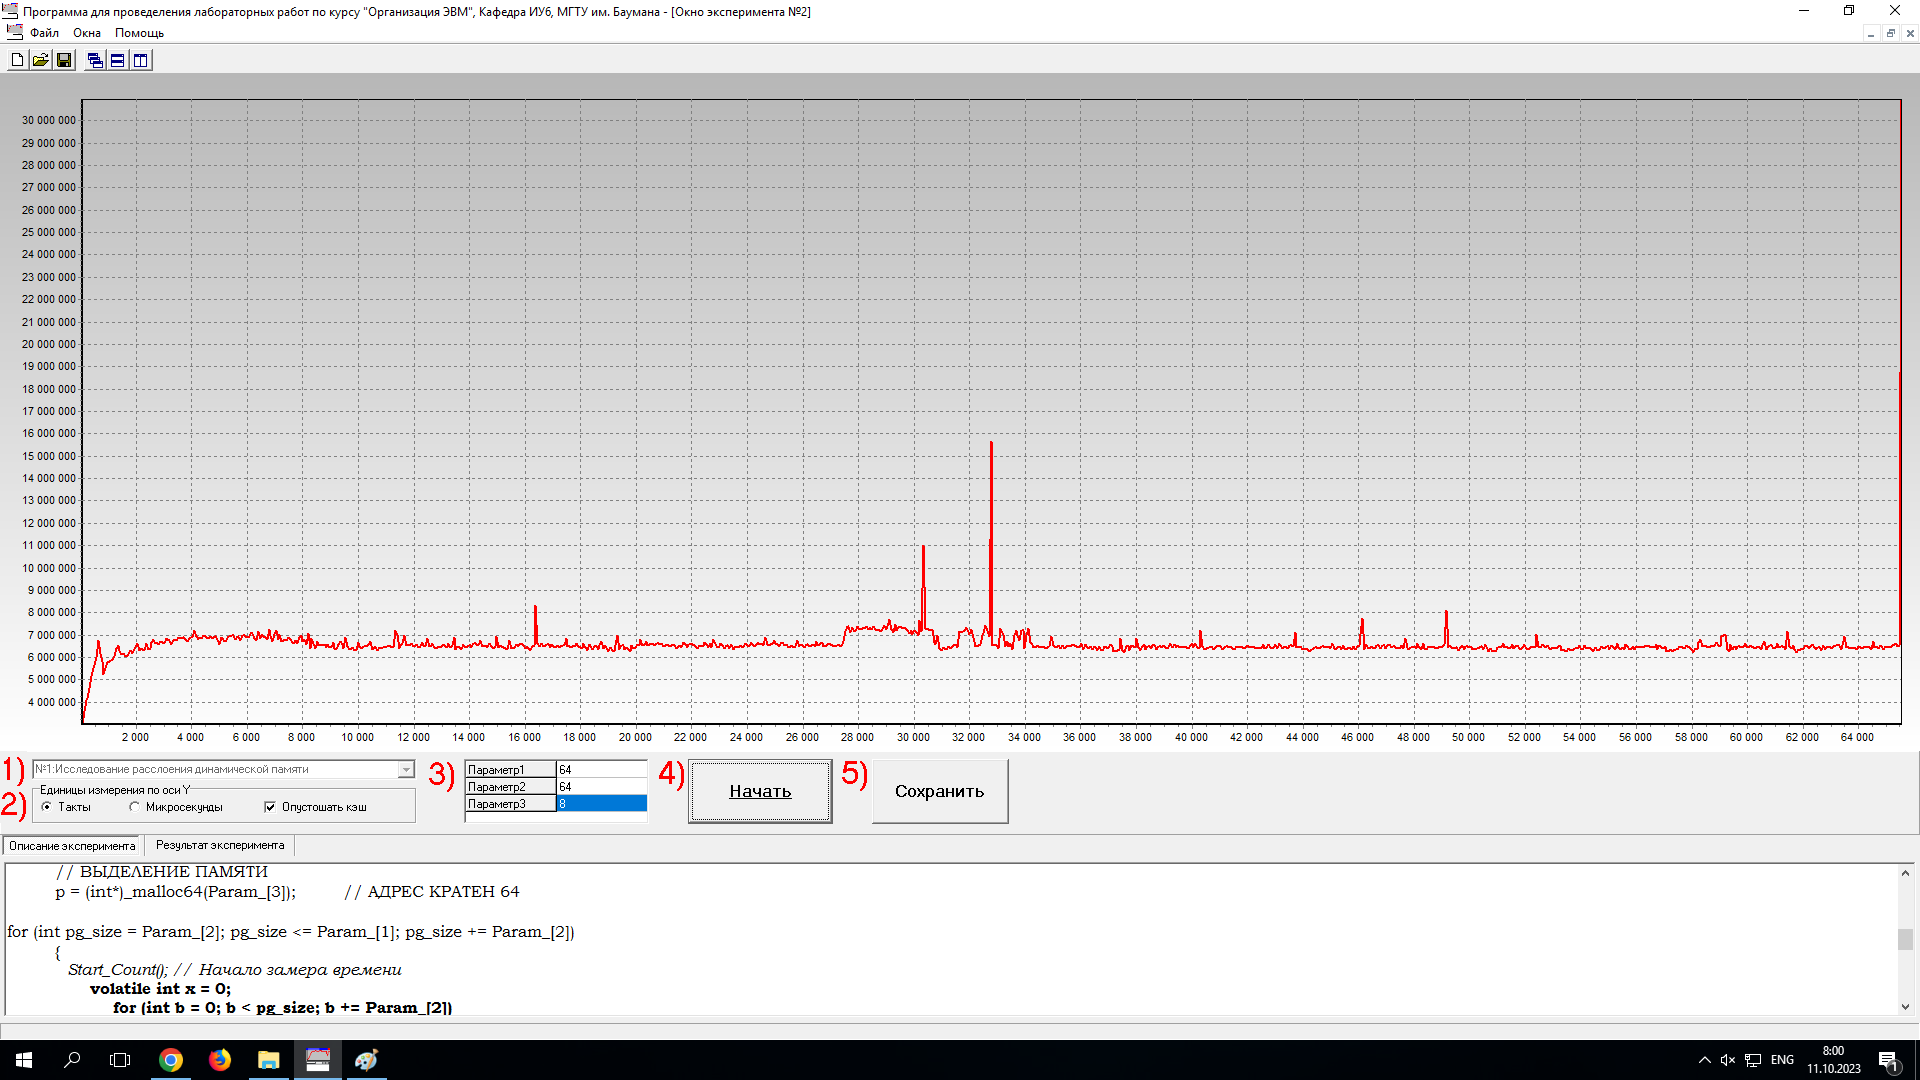
\includegraphics[width=1\textwidth]{img/1.png}
    \caption{Исследование расслоения динамической памяти}
	\label{fig:1}
\end{figure}

% \subsection{Цель эксперимента}

% \subsection{Описание проблемы}

% \subsection{Суть эксперимента}

% \subsection{Условия эксперимента}

% \subsection{Результаты эксперимента}

% \subsection{Вывод}

\newpage

\section{Эксперимент 2: Сравнение эффективности ссылочных и векторных структур}

\subsection{Параметры эксперимента}

\begin{enumerate}
    \item Параметр 1 (количество элементов в списке): 1
    \item Параметр 2 (максимальная фрагментация списка): 256
    \item Параметр 3 (шаг изменения фрагментации): 4
\end{enumerate}

\subsection{Результат эксперимента}

\begin{figure}[H]
	\centering
	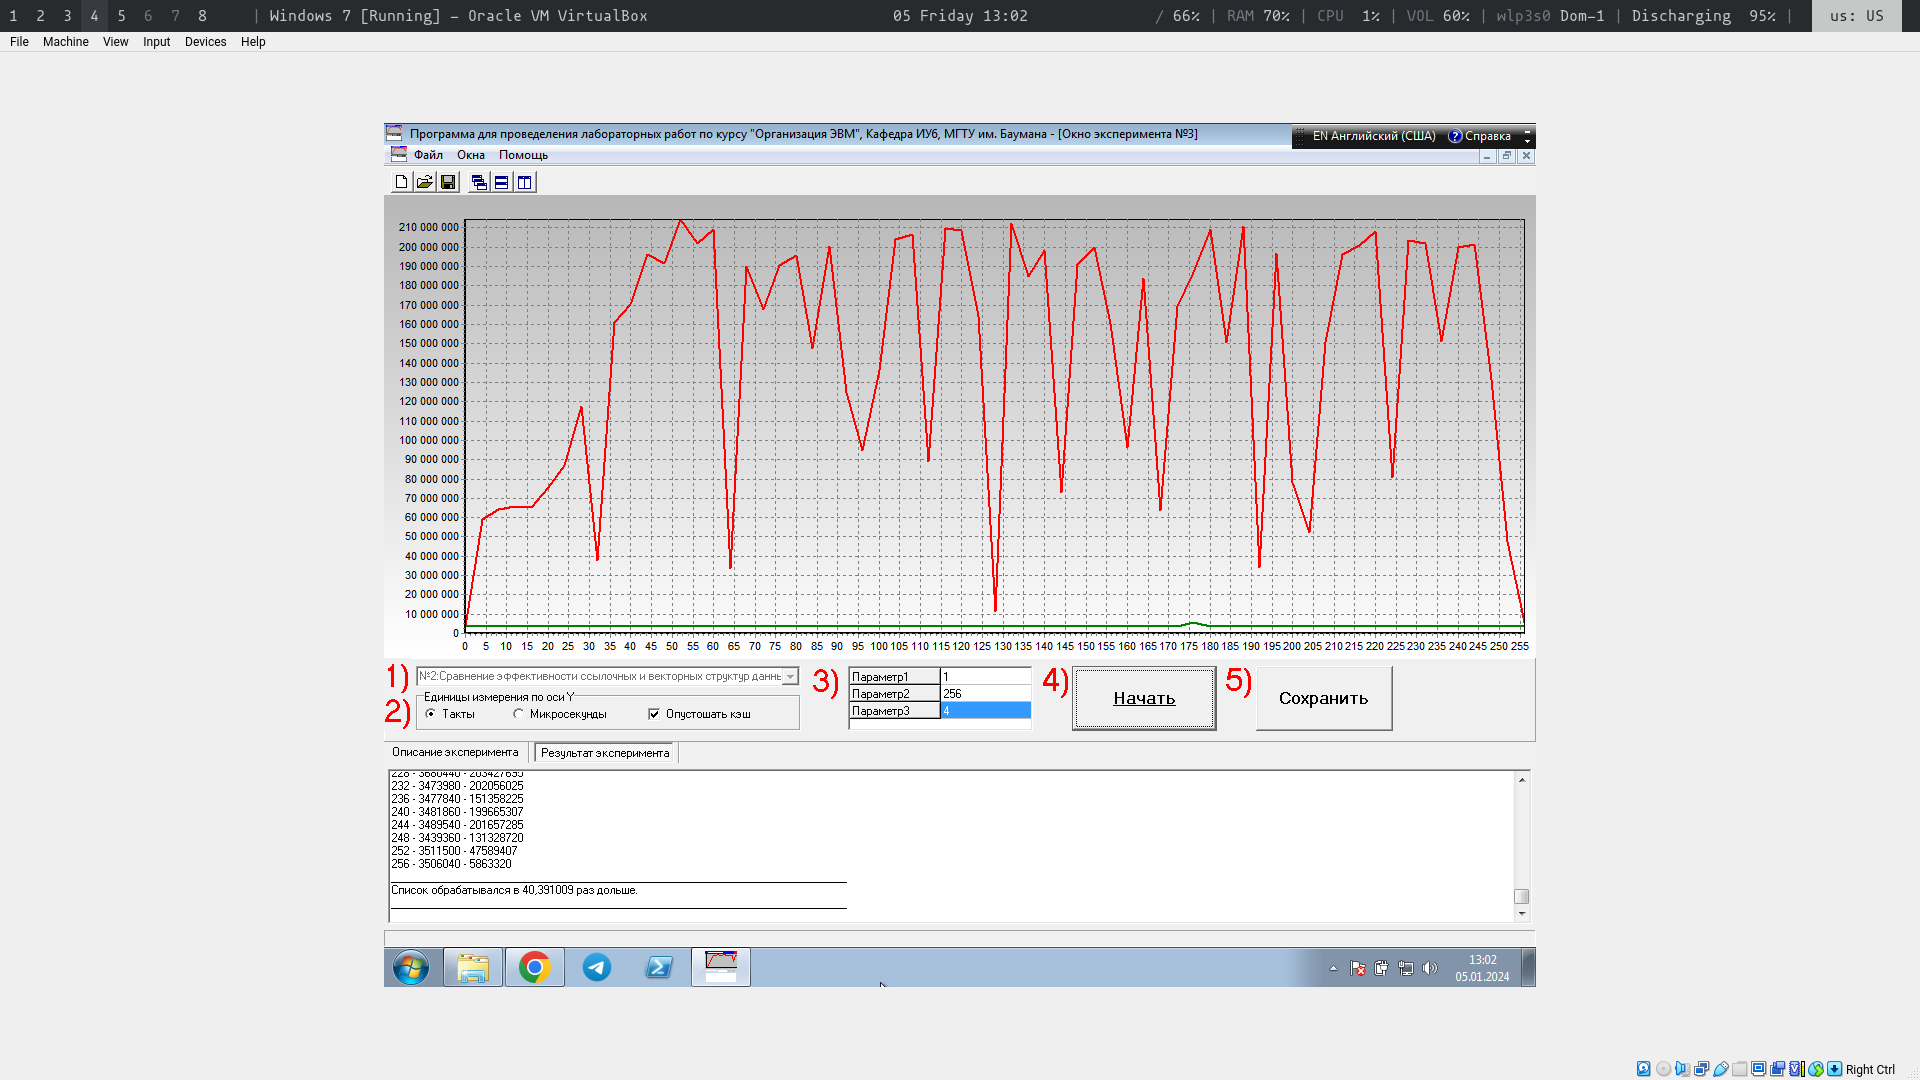
\includegraphics[width=1\textwidth]{img/2.png}
    \caption{Сравнение эффективности ссылочных и векторных структур}
	\label{fig:2}
\end{figure}

Список обрабатывался в 40.391009 раз дольше.

% \subsection{Цель эксперимента}

% \subsection{Описание проблемы}

% \subsection{Суть эксперимента}

% \subsection{Условия эксперимента}

% \subsection{Результаты эксперимента}

% \subsection{Вывод}

\newpage

\section{Эксперимент 3: Исследование эффективности программной предвыборки}

\subsection{Параметры эксперимента}

\begin{enumerate}
    \item Параметр 1 (шаг увеличения расстояния между читаемыми данными): 256
    \item Параметр 2 (размер массива): 512
\end{enumerate}

\subsection{Результат эксперимента}

\begin{figure}[H]
	\centering
	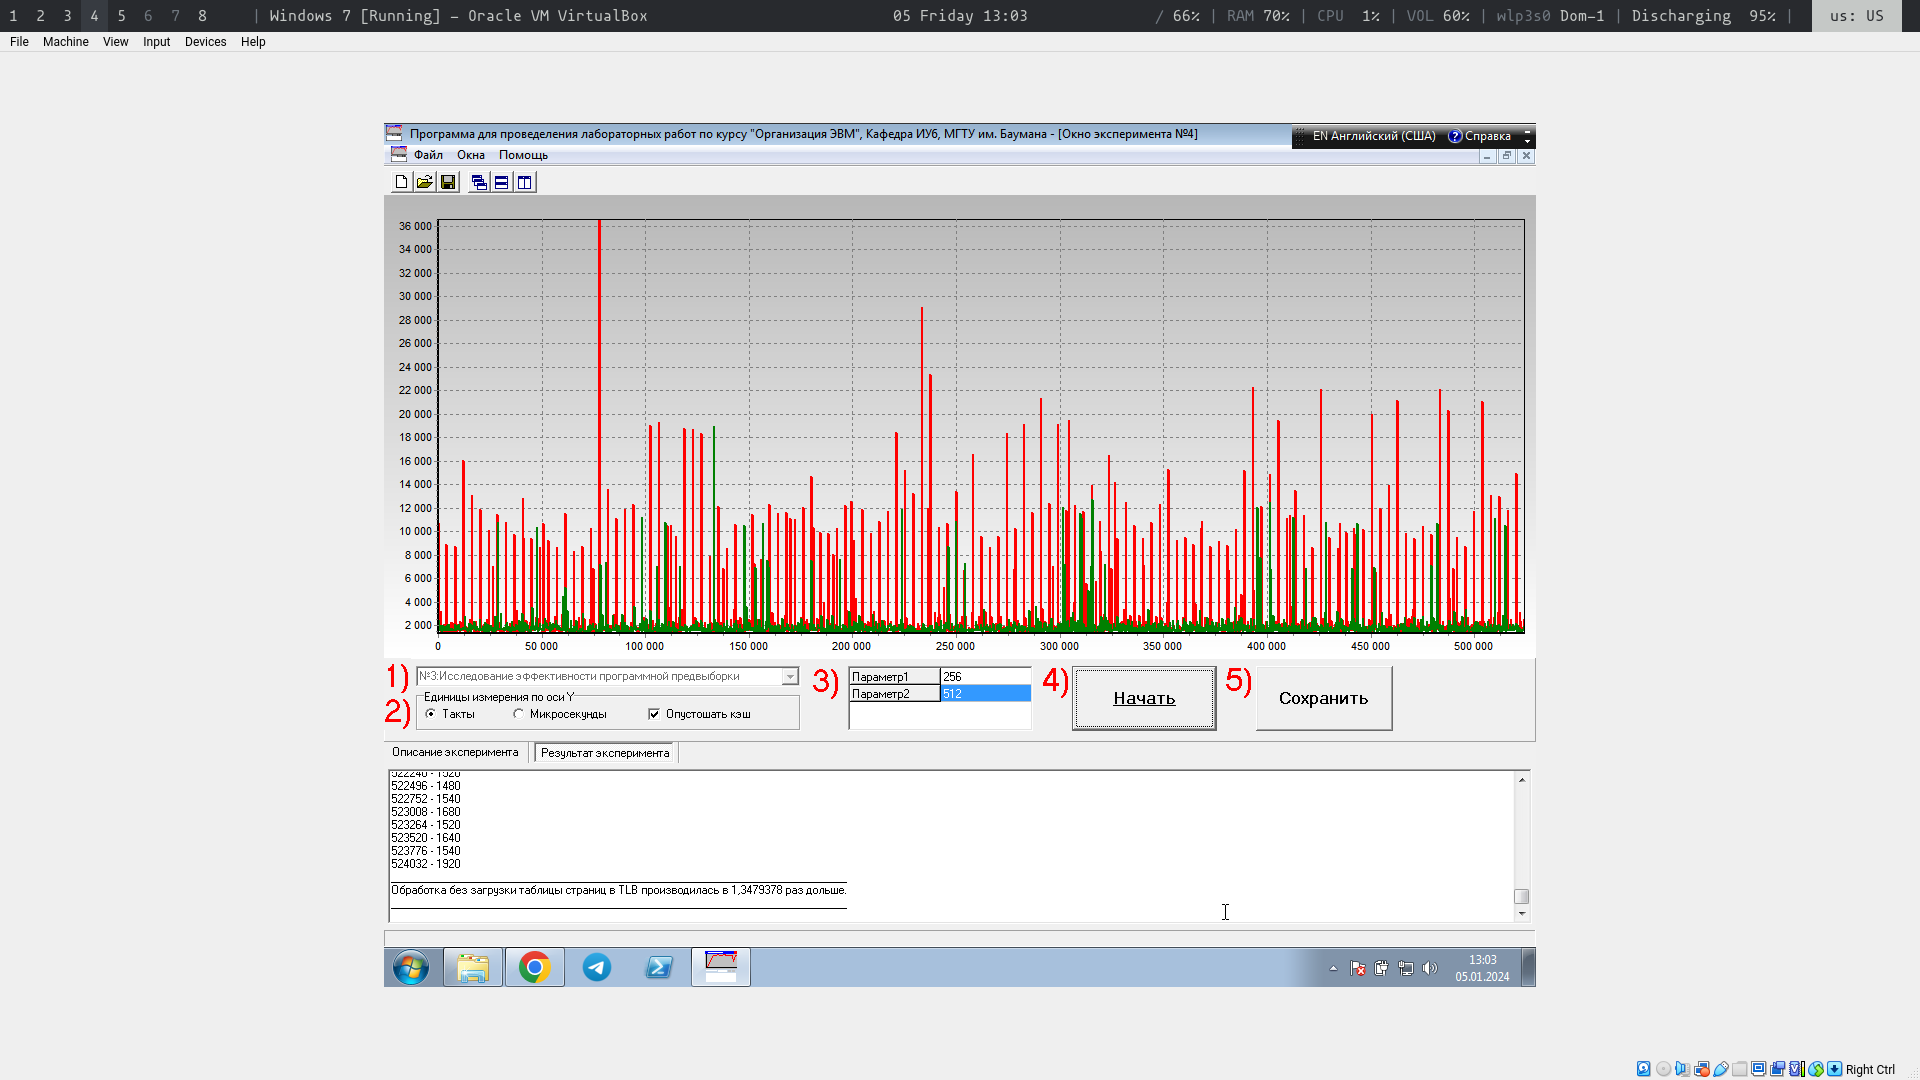
\includegraphics[width=1\textwidth]{img/3.png}
    \caption{Исследование эффективности программной предвыборки}
	\label{fig:3}
\end{figure}

Обработка без загрузки таблицы страниц в TLB производилась в 1.347938 раз дольше.

% \subsection{Цель эксперимента}

% \subsection{Описание проблемы}

% \subsection{Суть эксперимента}

% \subsection{Условия эксперимента}

% \subsection{Результаты эксперимента}

% \subsection{Вывод}

\newpage

\section{Эксперимент 4: Исследование способов эффективного чтения оперативной памяти}

\subsection{Параметры эксперимента}

\begin{enumerate}
    \item Параметр 1 (размер массива): 4
    \item Параметр 2 (количество потоков данных): 64
\end{enumerate}

\subsection{Результат эксперимента}

\begin{figure}[H]
	\centering
	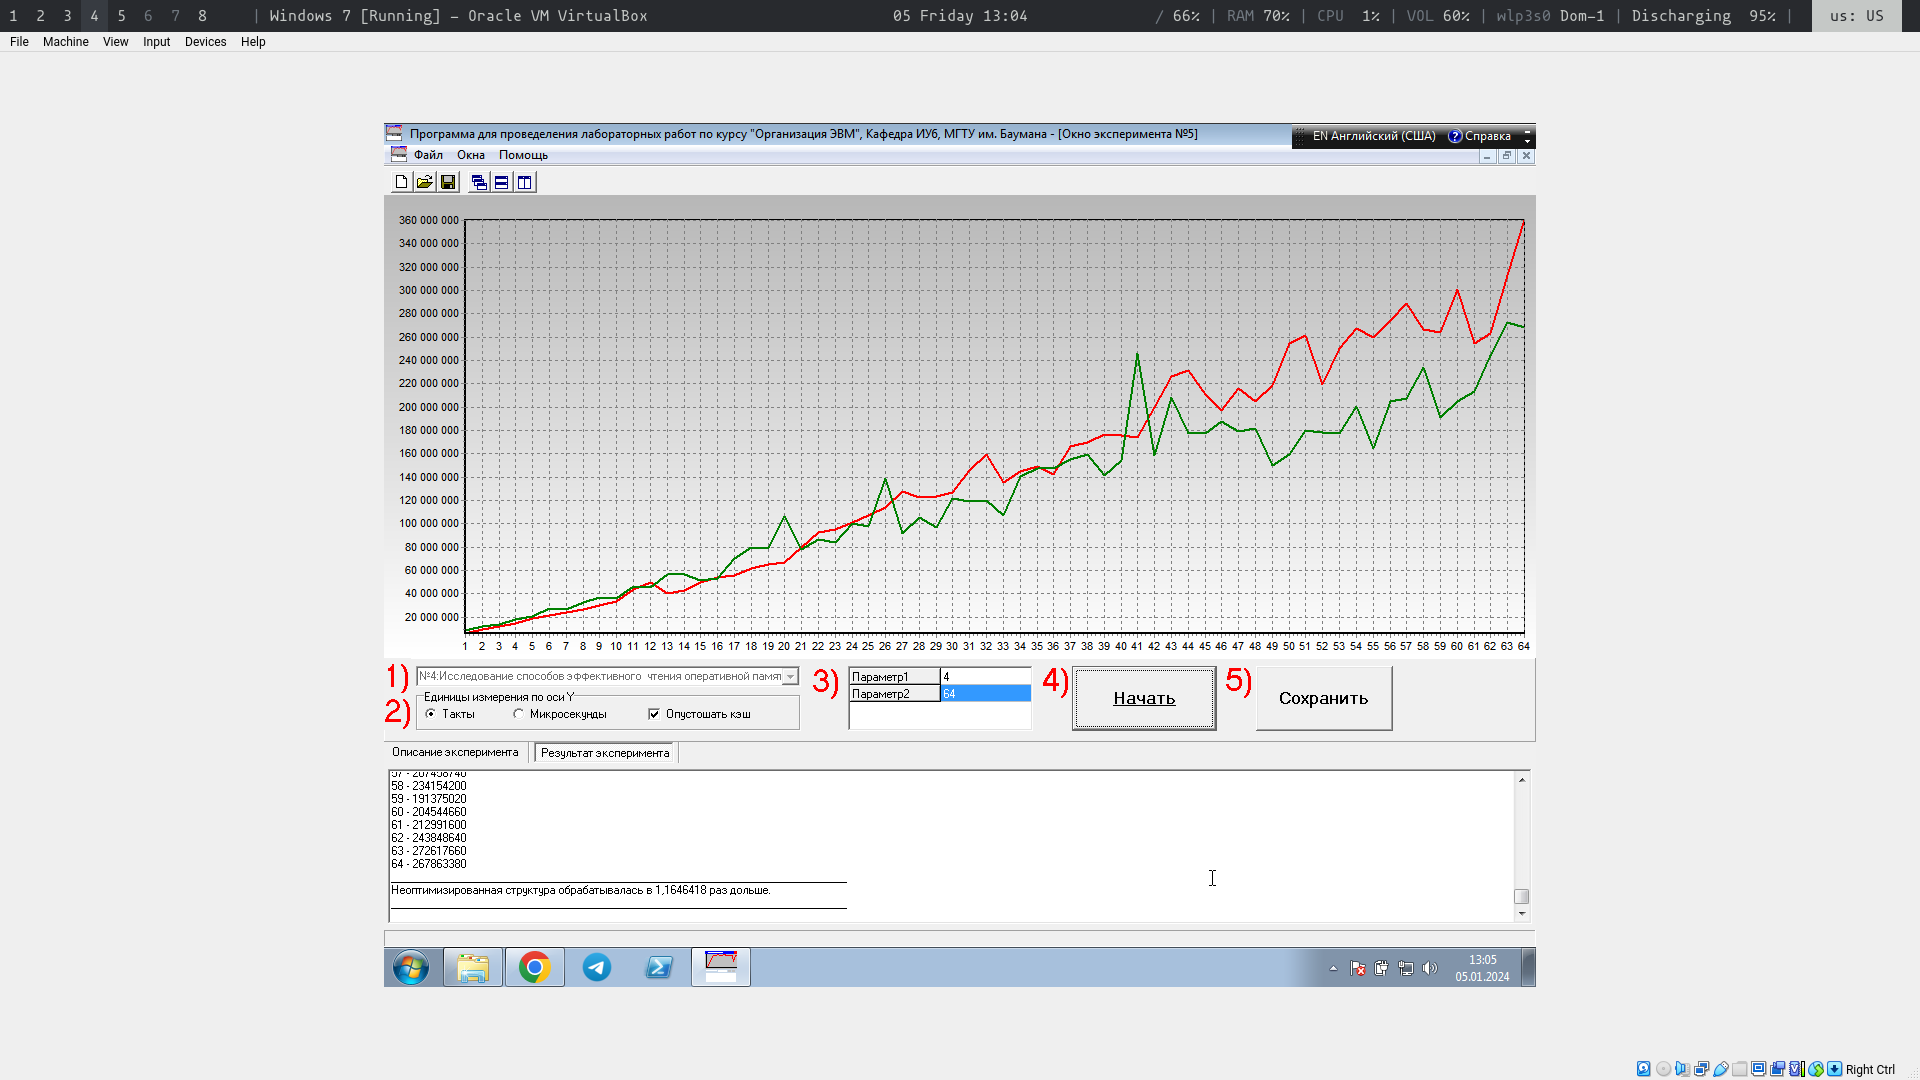
\includegraphics[width=1\textwidth]{img/4.png}
    \caption{Исследование способов эффективного чтения оперативной памяти}
	\label{fig:4}
\end{figure}

Неоптимизированная структура обрабатывалась в 1.1646418 раз дольше.

% \subsection{Цель эксперимента}

% \subsection{Описание проблемы}

% \subsection{Суть эксперимента}

% \subsection{Условия эксперимента}

% \subsection{Результаты эксперимента}

% \subsection{Вывод}

\newpage

\section{Эксперимент 5: Исследование конфликтов в кеш-памяти}

\subsection{Параметры эксперимента}

\begin{enumerate}
    \item Параметр 1 (размер блока кеш-памяти): 256
    \item Параметр 2 (размер линейки кеш-памяти): 128
    \item Параметр 3 (количество читаемых линеек): 512
\end{enumerate}

\subsection{Результат эксперимента}

\begin{figure}[H]
	\centering
	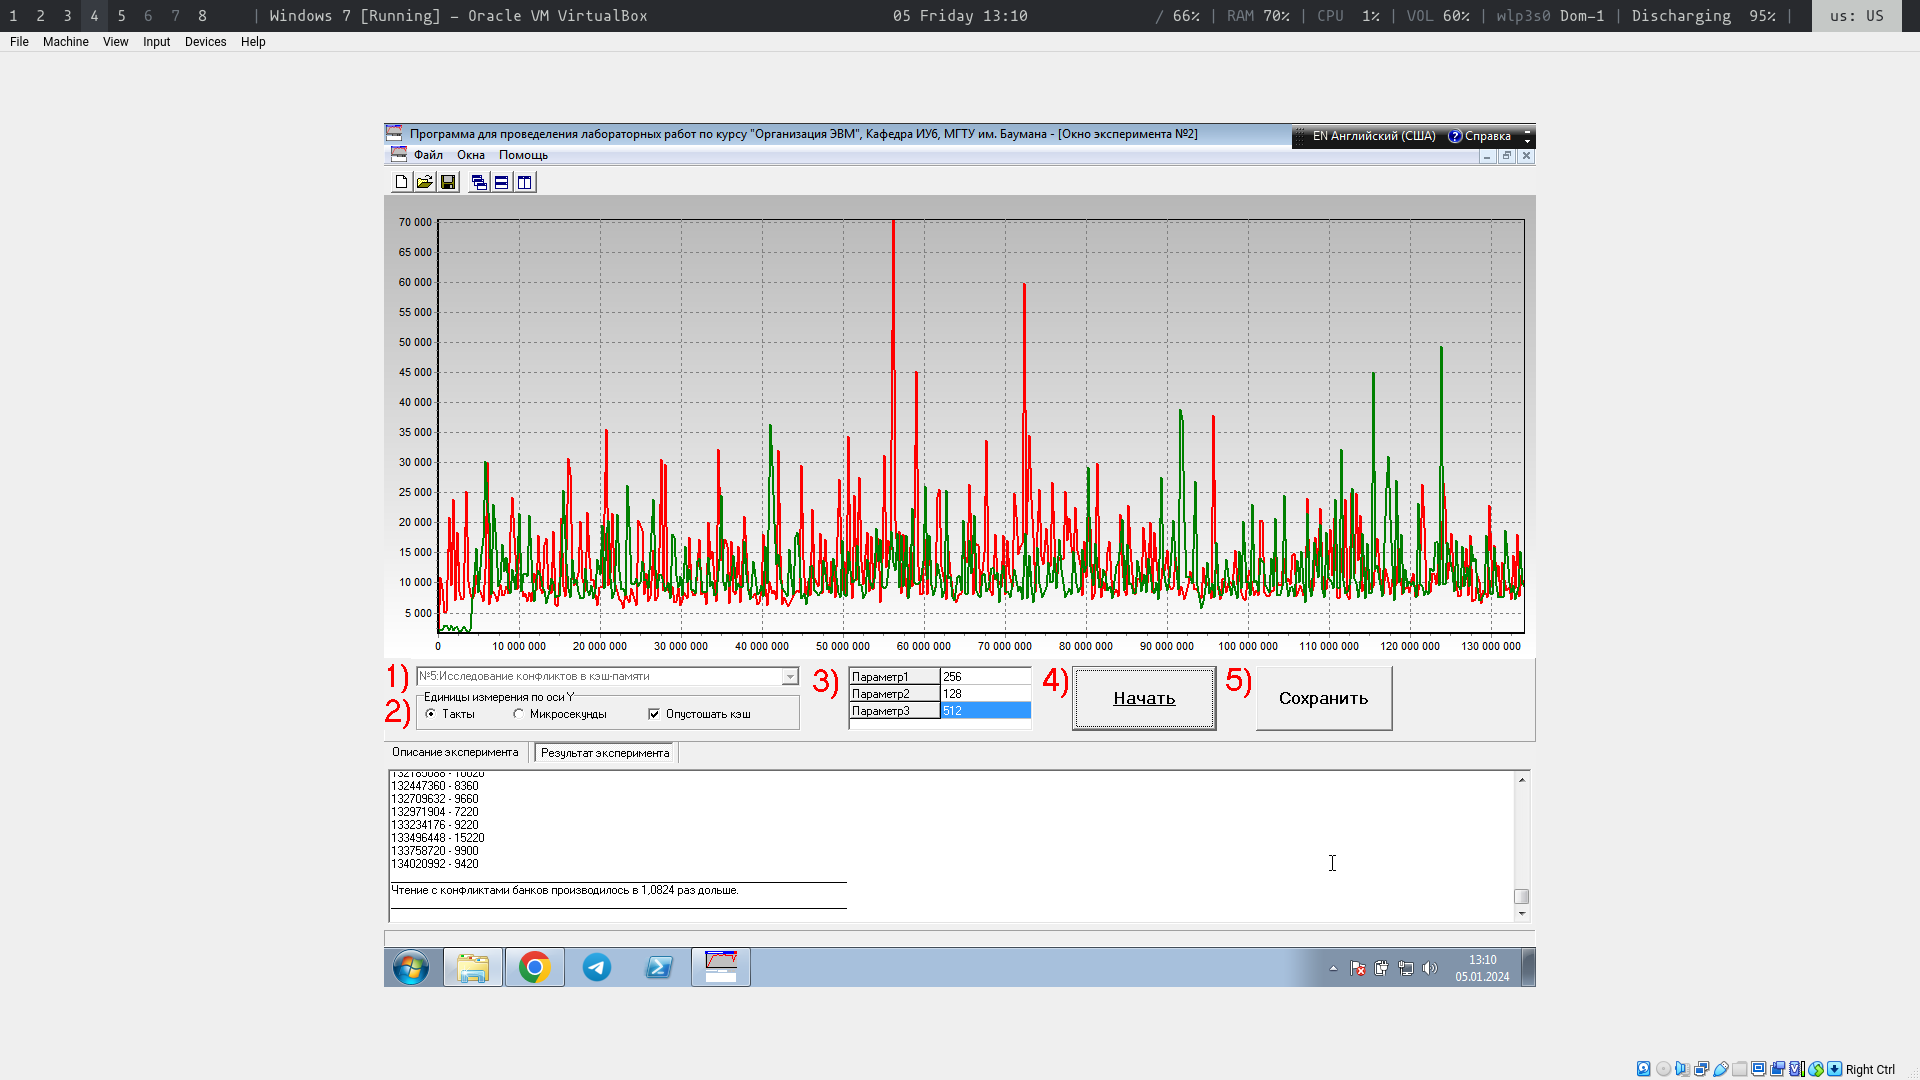
\includegraphics[width=1\textwidth]{img/5.png}
    \caption{Исследование конфликтов в кеш-памяти}
	\label{fig:5}
\end{figure}

Чтение с конфликтами банков производилось в 1.0824 раз дольше.

% \subsection{Цель эксперимента}

% \subsection{Описание проблемы}

% \subsection{Суть эксперимента}

% \subsection{Условия эксперимента}

% \subsection{Результаты эксперимента}

% \subsection{Вывод}

\newpage

\section{Эксперимент 6: Сравнение алгоритмов сортировки}

\subsection{Параметры эксперимента}

\begin{enumerate}
    \item Параметр 1 (количество 64-х разрядных элементов массивов): 1
    \item Параметр 2 (шаг увеличения размера массива): 4
\end{enumerate}

\subsection{Результат эксперимента}

\begin{figure}[H]
	\centering
	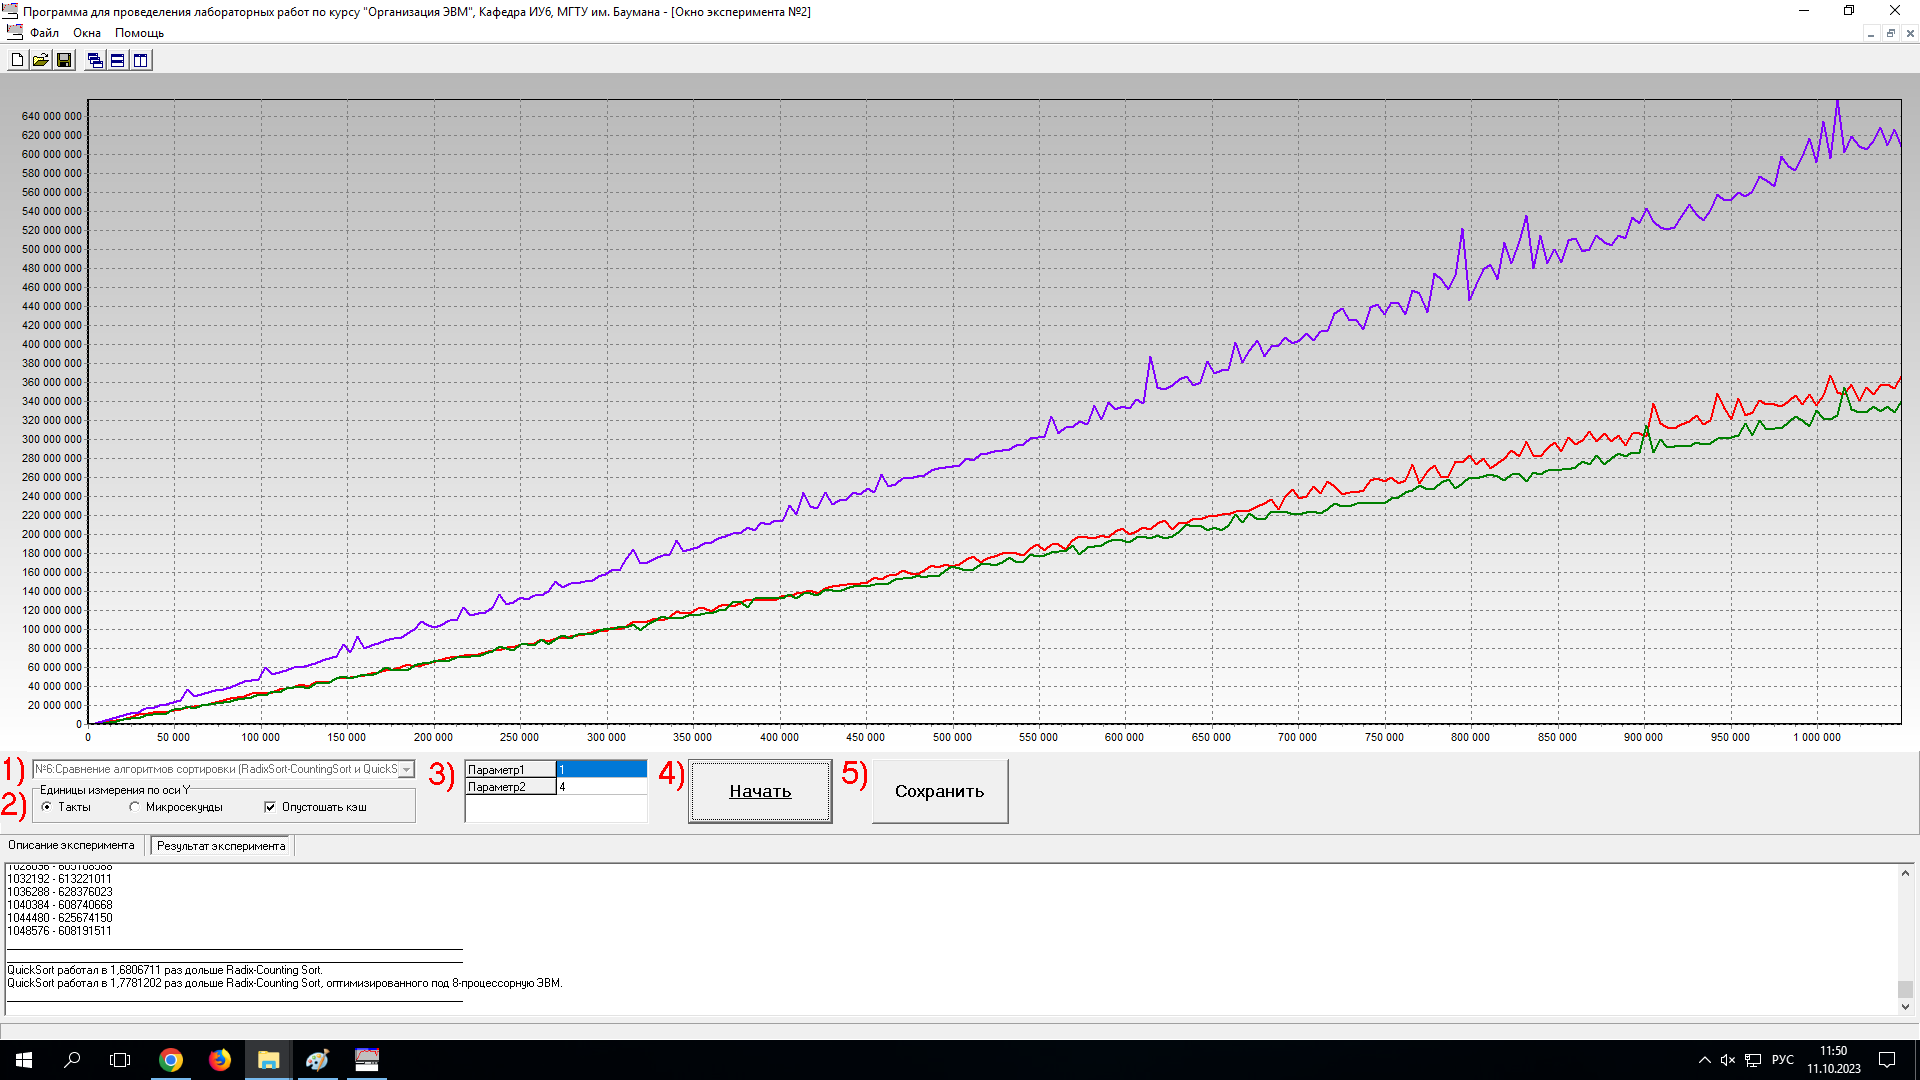
\includegraphics[width=1\textwidth]{img/6.png}
    \caption{Сравнение алгоритмов сортировки}
	\label{fig:6}
\end{figure}

QuickSort работал в 1.6806711 раз дольше Radix-Counting Sort.
QuickSort работал в 1.7781202 раз дольше Radix-Counting Sort, оптимизированного под 8-процессорную ЭВМ.

% \subsection{Цель эксперимента}

% \subsection{Описание проблемы}

% \subsection{Суть эксперимента}

% \subsection{Условия эксперимента}

% \subsection{Результаты эксперимента}

% \subsection{Вывод}

% \begin{figure}[H]
% 	\centering
% 	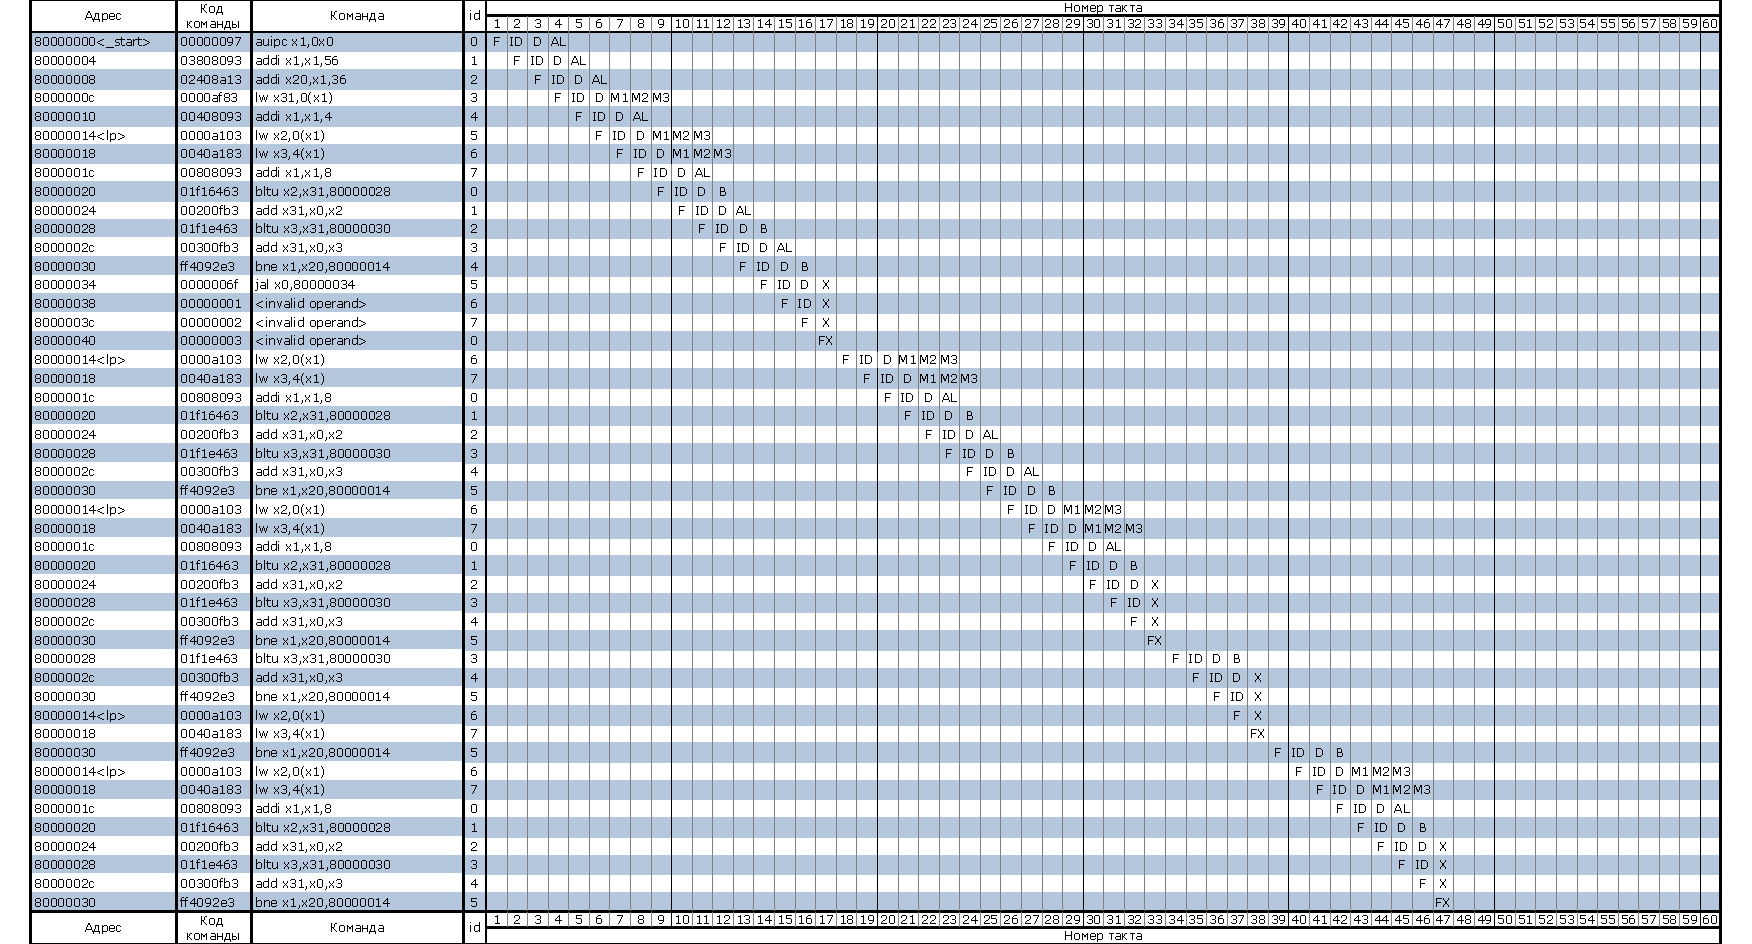
\includegraphics[width=1\textwidth]{img/pipeline-optimized.pdf}
%     \caption{Трасса выполнения оптимизированной программы}
% 	\label{fig:po}
% \end{figure}

\newpage

\phantomsection\section*{ЗАКЛЮЧЕНИЕ}\addcontentsline{toc}{section}{ЗАКЛЮЧЕНИЕ}

Освоены принципы эффективного использования подсистемы памяти современных универсальных ЭВМ, обеспечивающей хранение и своевременную выдачу команд и данных в центральное процессорное устройство.
Работа была проведена с использованием программы для сбора и анализа производительности PCLAB.
Поставленная цель достигнута.

\end{document}
